\chapter{Benchmark}
\label{chapter:benchmark}

We built a benchmark framework to efficiently and robustly conduct experiments with many different
preprocessing methods over many datasets reporting as many evaluation metrics as supplied. The core
idea of the framework is depicted in Figure~\ref{figure:framework}. In its simplest form, the
framework performs a single run for every combination of a dataset and a preprocessing method. In
each run, a preprocessing method is applied to the training part of a dataset, yielding a new
resampled training set, which is then passed to the AutoML component of the framework. We use a
state-of-the-art AutoML framework called Auto-Sklearn~\cite{auto-sklearn-1.0} for selecting,
training and tuning a classifier suitable for a given dataset. We provide more details about
Auto-Sklearn in section~\ref{section:auto-sklearn}. Once a classifier has been trained, we perform
predictions using unseen examples from the test set and report evaluation scores achieved. We use
an open-source tool called Mlflow~\cite{mlflow} to facilitate storing and displaying various
information about each run, such as hyperparameters, scores and performance graphs, through a
user-friendly web interface.

Additionally, the framework supports hyperparameter tuning of preprocessing methods using a grid
search. As every preprocessing method comes with a set of hyperparameters to tune, such as the
number of neighbours in methods employing KNN, the number of clusters in KMeans or desired
imbalance ratio after resampling, we provide an interface for supplying these hyperparameters and
use them to find the best performing combination. In such cases, the framework runs every
combination of a dataset, a preprocessing method and an instantiation of its hyperparameters,
reporting each run separately to Mlflow. We can use Mlflow's functionality to present, filter and
compare different runs to see which hyperparameters combination resulted in the best performance.

Performing a grid search over datasets, preprocessing methods and their hyperparameters requires a
tremendous amount of computation time and memory, and is usually run on large computational
clusters spanning multiple machines. Our framework is able to work in multi-node environments by
checking if a given combination of a dataset, a preprocessing method and its hyperparameters is
already finished, running or failed, or has not been executed at all, and reacts accordingly. This
prevents multiple instances from executing the same runs. By default, a given run is skipped if it
has successfully been completed or is currently running. Each instance communicates with the same
Mlflow tracking server allowing the instances to share information about finished, running and
failed runs. A user can observe the same information from Mlflow's web interface in real-time. A
by-product of this functionality is the ability to re-run a subset of runs which have not been
attempted in case of power failure or any other failure that halted the execution.

\begin{figure}
    \centering
    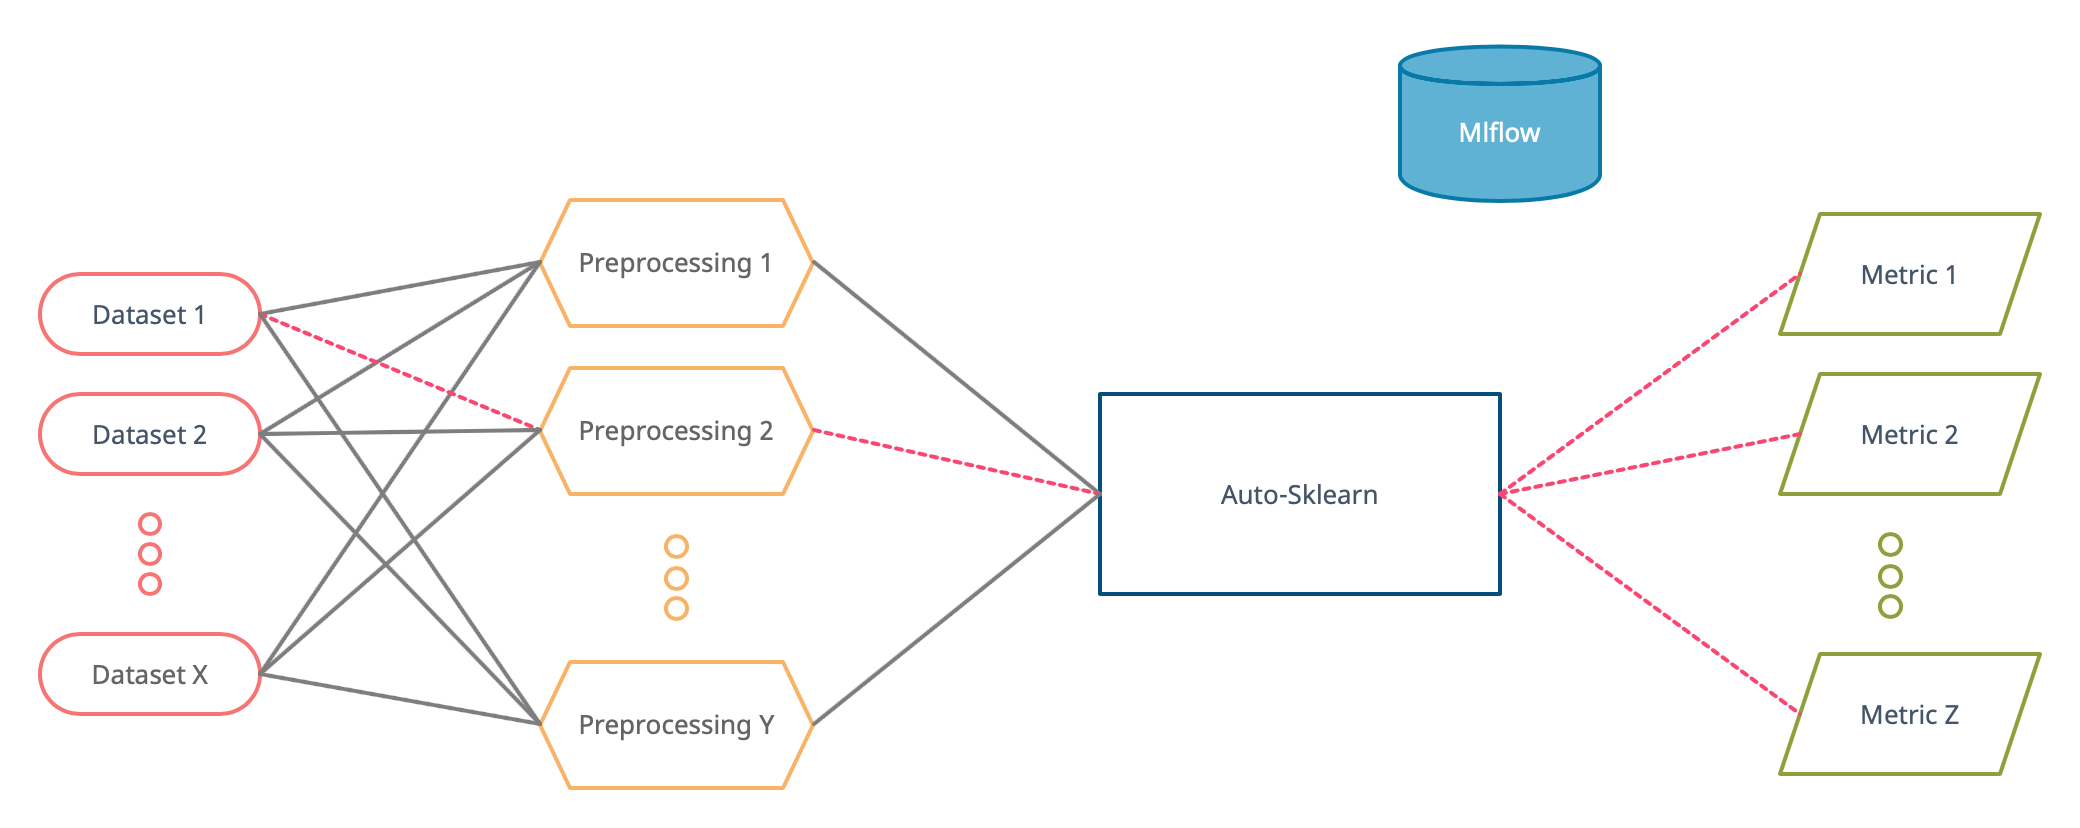
\includegraphics[width=\linewidth]{figures/diagram.png}
    \caption{
        \textbf{Flowchart Showing Rough Sketch of the Framework}. The figure shows how each
        combination of a dataset, a preprocessing method, and optionally, the method's
        hyperparameters is executed, producing a set of specified metrics on the output.
        Information about each stage of the run is stored in Mlfow, allowing user-friendly
        observation, filtering and comparison of runs.
    }
    \label{figure:framework}
\end{figure}


\section{Benchmark Setup}
\label{subsection:benchmark}

We ran an extensive benchmark covering sixteen preprocessing methods discussed in
Chapter~\ref{chapter:imb-classif} and one no-op baseline method. We covered a large number of
possible hyperparameter configurations for each method shown in Table~\ref{table:configs}. All
preprocessing methods used in the benchmark come from the Imbalanced Learn
library~\ref{section:imblearn}. Every preprocessing method was run on seventeen public and
proprietary datasets shown in Table~\ref{table:datasets}. We used 75\% of data samples from each
dataset as a training set and the remaining 25\% as a testing set. The split was done to retain the
original imbalance in both sets.

We utilised the state-of-the-art AutoML system Auto-Sklearn~\ref{section:auto-sklearn} to find,
train and tune the best performing classifier on the training set using five-fold cross-validation
as the validation technique. Auto-Sklearn was set to optimise the ROC AUC
score~\ref{subsection:roc}. Each run was initially given a total of 30 minutes for training on
public datasets; a single machine learning model had 10 minutes to finish training. Failed runs
were subsequently given 45 minutes in total, and each model had 20 minutes to finish. Runs that
were still unsuccessful even after increasing the amount of time for the training were not repeated
anymore. It was sufficient to dedicate only five minutes to Auto-Sklearn on proprietary datasets
due to their sizes, and no repetitions were needed. We did not limit the time for preprocessing
step in any way to obtain data about the performance of preprocessing methods on datasets of
different sizes.


\section{Auto-Sklearn}
\label{section:auto-sklearn}

Auto-Sklearn~\cite{auto-sklearn-1.0}, as its authors say, frees its users from model selection and
hyperparameter tuning. It builds on top of the famous machine learning library called
Scikit-Learn~\cite{sklearn}. We utilise Auto-Sklearn as the backbone of our experiment precisely
for these reasons. It allows us to forget about selecting the most suitable model and tuning the
model's hyperparameters for the given dataset allowing us to focus on the problem of imbalanced
learning more deeply. We chose Auto-Sklearn for its significantly better performance than other
competing AutoML systems~\cite{auto-sklearn-1.0}. Although the second version of Auto-Sklearn,
bringing substantial advances~\cite{auto-sklearn-2.0}, has been available since 2020, we chose not
to use it as it is still in an experimental phase and may contain undiscovered bugs.

Auto-Sklearn extends existing AutoML architectures utilising the Bayesian optimiser by using
meta-learning and ensemble building to further boost a system's performance. The overall workflow
of Auto-Sklearn can be seen in Figure~\ref{figure:auto-sklearn}. We will briefly explain how each
of the components works and provide comments in cases where we have needed to tweak the behaviour
of Auto-Sklearn to allow complete control over the experiment.

\begin{figure}
    \centering
    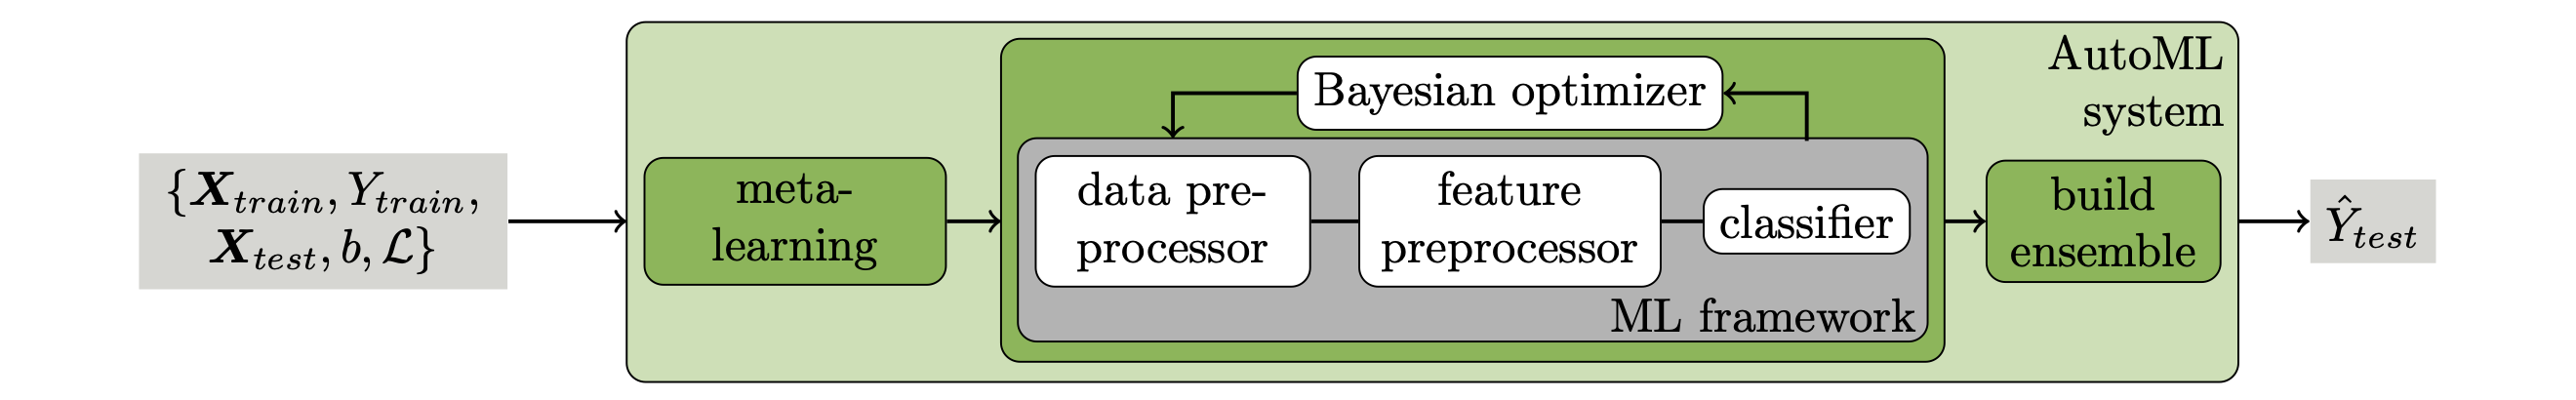
\includegraphics[width=\linewidth]{figures/auto-sklearn.png}
    \caption{
        \textbf{Auto-Sklearn's workflow~\cite{auto-sklearn-1.0}.} This figure depicts how
        Auto-Sklearn finds, tunes and trains an ensemble of models giving the best performance
        using the training portion of labeled data while respecting budget constraints.
        Subsequently it produces predictions for the testing portion of data. All of this happens
        in a single call to Auto-Sklearn's \texttt{fit} method.
    }
    \label{figure:auto-sklearn}
\end{figure}

\begin{itemize}

    \item \textbf{\emph{Meta-learning}} uses previous knowledge stored in a \emph{knowledge base}
        consisting of pairs of dataset characteristics and a machine learning model +
        hyperparameters exhibiting the best performance on that dataset to suggest models that are
        likely to perform well on a new dataset. Characteristics are viewed as vectors living in a
        normed meta-features vector space allowing us to use a notion of distance between datasets
        to find similar ones and use models that performed well on those datasets as a starting
        point for further tuning. Auto-Sklearn built a knowledge base consisting of 140 datasets
        from OpenML~\cite{openml}. They extracted easy-to-compute characteristics combined with a
        machine learning model performing best on the given dataset. This way, Auto-Sklearn can
        quickly suggest configurations that are likely to perform well on a new dataset to the
        Bayesian optimiser. Unfortunately, we encountered various errors with meta-learning and
        could not get it to work correctly, so we disabled it entirely for our experiment.

    \item \textbf{\emph{Bayesian optimisation}} serves as an intelligent random search for
        hyperparameter tuning. It is a powerful technique suitable for finding the extrema of
        objective functions expensive to evaluate, such as tuning hyperparameters in a machine
        learning model, in as few sampling steps as possible~\cite{bayesian-opt}. We can formulate
        the hyperparameter tuning of a model $\mathcal{M}$ as a function $f \colon \mathbb{R}^d \to
        \mathbb{R}$. The domain of $f$ is a vector space containing possible configurations of
        hyperparameters. The output of $f$ is a performance of model $\mathcal{M}$ evaluated using
        some evaluation function $\mathcal{F}$. Evaluating $f$ is an expensive operation as it may
        include training a deep neural network, for example. Bayesian optimisation fits a
        probabilistic model capturing a relationship between hyperparameters and model performance.
        The probabilistic model suggests a promising configuration of hyperparameters based on its
        current beliefs. It evaluates the model using these hyperparameters and uses the results to
        update its beliefs in a loop. It can explore new regions and exploit known regions to boost
        performance further~\cite{auto-sklearn-1.0}.

    \item \textbf{\emph{Ensemble building}} is a process of combining several models to achieve
        better overall performance. It is well known that ensembles outperform individual models,
        and combining multiple strong models with uncorrelated errors leads to exceptionally high
        performance~\cite{auto-sklearn-1.0}. Auto-Sklearn stores models trained during the bayesian
        optimisation step and constructs an ensemble out of them to achieve even better
        performance. To reduce the framework's complexity and allow for more straightforward
        reasoning about performance, we disable automatic ensemble building in Auto-Sklearn.

    \item \textbf{\emph{Data preprocessing \& Feature preprocessing}} are two distinct steps
        focusing on data preparation and feature engineering, respectively. The data preprocessing
        step consists of a combination of steps such as missing values imputation, one-hot
        encoding, data normalisation, scaling and centring. On the other hand, feature
        preprocessing tries to create new features using polynomial features or select a subset of
        features using Principal Component Analysis (PCA) or Independent Component Analysis (ICA).
        Another thing Auto-Sklearn sometimes chooses to do is balancing. Balancing adjusts the
        weights of individual classes to punish misclassification of a particular class more than
        misclassification of other ones. Balancing is essentially the same as if we applied Random
        Oversampling discussed in Chapter~\ref{chapter:imb-classif}. We disabled balancing, data
        and feature preprocessing steps altogether to gain complete control over the experiments.
        We apply the same data preprocessing steps to all datasets, and we do not perform any
        feature preprocessing. Balancing is entirely disabled as it would not provide the same
        conditions to all preprocessing methods.

    \item \textbf{\emph{Classifiers.}} Auto-Sklearn uses a list of 15 classification algorithms to
        choose from. The list consists of general linear models, support vector machines, nearest
        neighbours, naive Bayes and decision trees~\cite{auto-sklearn-1.0}. We have excluded
        Multi-Layer Perceptron from the list as it consumes a significant amount of resources
        during training, and the tabular datasets used in the experiment do not require the use of
        neural networks~\cite{nn-for-tabular-data}.

\end{itemize}


\section{Imbalanced Learn}
\label{section:imblearn}

Imbalanced Learn~\cite{imblearn} is a library providing implementations of various imbalanced
preprocessing methods. All preprocessing methods share the same API inspired by
Scikit-Learn~\cite{sklearn}. We use this library to avoid reimplementing every preprocessing method
from scratch, as it would be time-consuming and error-prone. All preprocessing methods mentioned in
Chapter~\ref{chapter:imb-classif} are implemented in the Imbalanced Learn library.


\section{Mlflow}
\label{section:mlflow}

Mlflow~\cite{mlflow} is an open-source project aiming to provide a unified interface for storing,
comparing, deploying and managing machine learning workflows. It natively integrates with many
popular machine learning libraries such as Scikit-Learn, PyTorch, Tensorflow and many others.
Although it does not support Auto-Sklearn explicitly, we used the fact that Auto-Sklearn builds on
top of Scikit-Learn to incorporate Mlflow into our framework. We log all helpful information about
each run of an experiment to Mlflow. Logged information includes information about the dataset,
hyperparameters of the preprocessing method used, Auto-Sklearn's hyperparameters, and information
about all models Auto-Sklearn trained during the run. We also include information such as the
performance of each model during cross-validation, the performance of the best model on the test
data, the duration of the preprocessing step and multiple automatically generated plots.


\section{OpenML}
\label{section:openml}

OpenML~\cite{openml} is an initiative to allow people to share high-quality resources and share
valuable information among the machine learning community. It provides approximately four thousand
datasets instantly available for use. OpenML provides rich metadata for each dataset allowing
automated processing and filtering of the datasets. We used OpenML and its Python API to select
imbalanced datasets suitable for use in the benchmark.
